\documentclass[addpoints,12pt]{exam} %answers 
\usepackage[paper=a4paper,left=15mm,right=15mm,top=25mm,bottom=25mm]{geometry}
\usepackage{graphicx}
%\usepackage[dvips]{graphicx}
\usepackage{floatflt,epsfig} 
\usepackage{ngerman}
\usepackage{german}
\usepackage[utf8]{inputenc}
\usepackage{amssymb, amsmath}
\usepackage[gate,ic,optics]{circ}
\usepackage{hyperref}

\usepackage{tikz,pgfplots}

\usepackage{graphicx}
%\usepackage{geometry}
\usepackage{calc}


\usepackage{qrcode} 
\usepackage{wrapfig}
\usepackage{gensymb}
\usepackage{siunitx}

\usepackage{color}
\definecolor{GridColor}{gray}{0.8}
\definecolor{SolutionBoxColor}{gray}{0.8}
\definecolor{SolutionColor}{rgb}{0.8,0.9,1}

\colorgrids
\colorsolutionboxes

%%MACROS 
\newcommand{\tdate}{22. Oktober 2021}
\newcommand{\myqr}{\qrcode[hyperlink, height = 1cm]{www.github.com/shahrrks}}
\newcommand\gauss[2]{1/(#2*sqrt(2*pi))*exp(-((x-#1)^2)/(2*#2^2))} % Gauss function, parameters mu and sigma
%%
\newcommand{\gr}{ETIT-1}

\sisetup{
locale = DE ,
per-mode = symbol
}

\pagestyle{headandfoot}

\headrule
\footrule
\firstpageheader{\gr}{\bfseries\Large {Übungsblatt 1}}{\tdate}
\runningheader{\gr}
{Übungsblatt - 1}
{\tdate}
\firstpagefooter{\gr}{Seite \thepage\ von \numpages}{\myqr}
\runningfooter{\gr}{Seite \thepage\ von \numpages}{Shah Rrks}

\boxedpoints
%\pointpoints{Punkt}{Punkte}
\pointsinmargin
\marginpointname{\%}

\begin{document}
%\setcounter{section}{1} %current page -1
\author{Shah Rrks}
\section*{Experimental Physik}
\begin{questions}
\question In der Abbildung unten sei x = 50m und h = 10m. Der Affe lässt sich genau in dem Moment fallen, in dem der Pfeil abgeschossen wird. Welche Abschussgeschwindigkeit muss der Pfeil mindestens haben, damit er den anfangs 11,2 m hoch sitzenden Affen erreicht, bevor dieser auf den Boden auftrifft?

\begin{figure}[h]
\centering
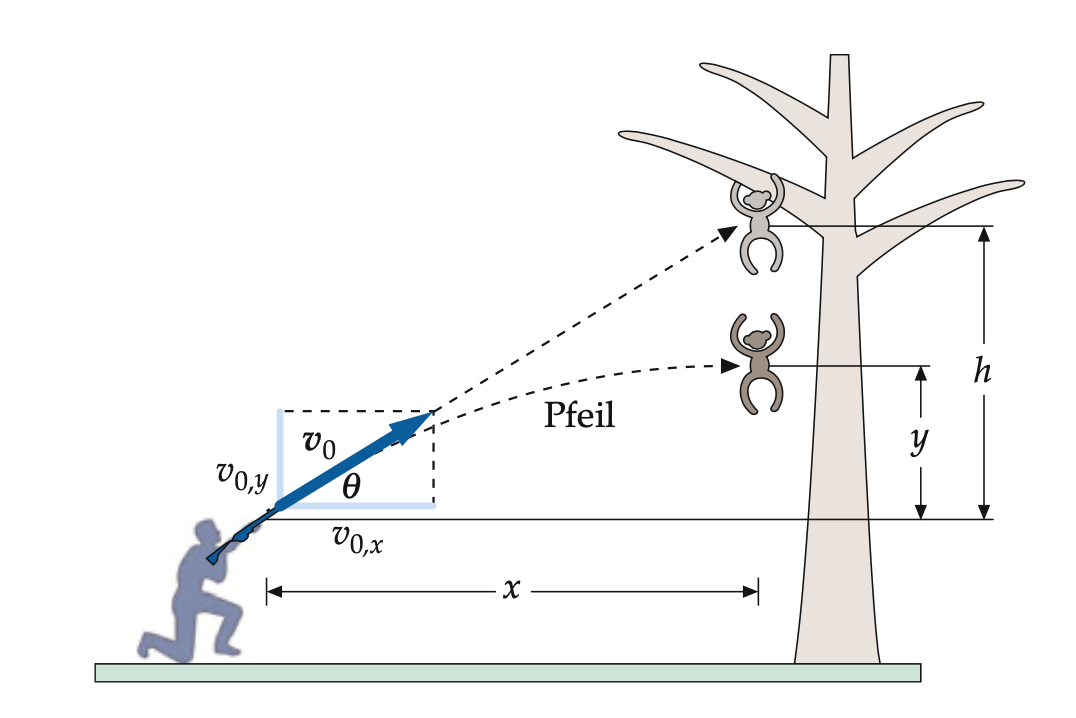
\includegraphics[width=0.7\textwidth]{auf1}
\end{figure}

\makeemptybox{4in}
\pagebreak
\question In den Abbildung unten welche Zügekräfte wirken in dem horizontalen Seil und in dem schrägen Seil



\begin{figure}[h]
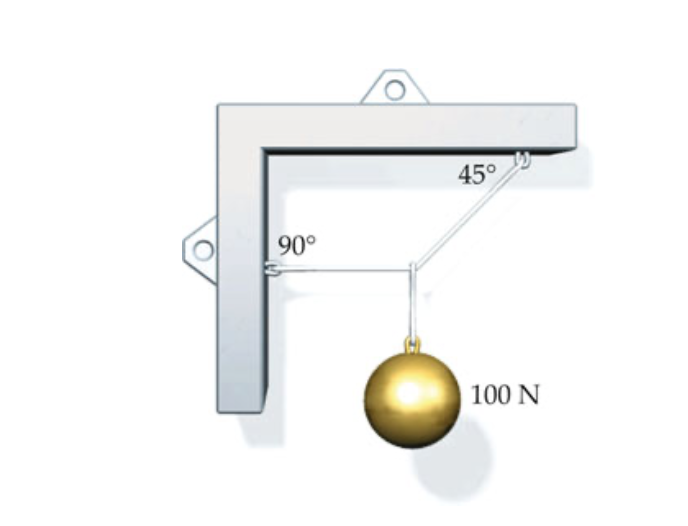
\includegraphics[width=0.5\textwidth]{auf2}
\label{fig:zu Aufgabe 2}
\end{figure}

\question Eine Verkehrsampel mit einer Masse von 35,0 kg ist, wie in Abbildung gezeigt, an zwei Drähten aufgehängt. a) Zeichnen Sie das Kräftediagramm und beantworten Sie an- hand dessen qualitativ die folgende Frage: Ist die Zugkraft im Draht 2 größer als die im Draht 1? b) Überprüfen Sie Ihre Ant- wort unter Anwendung der Newton’schen Axiome und durch Berechnen der beiden Zugkräfte.
\begin{figure}[h]
    \hspace{9cm}
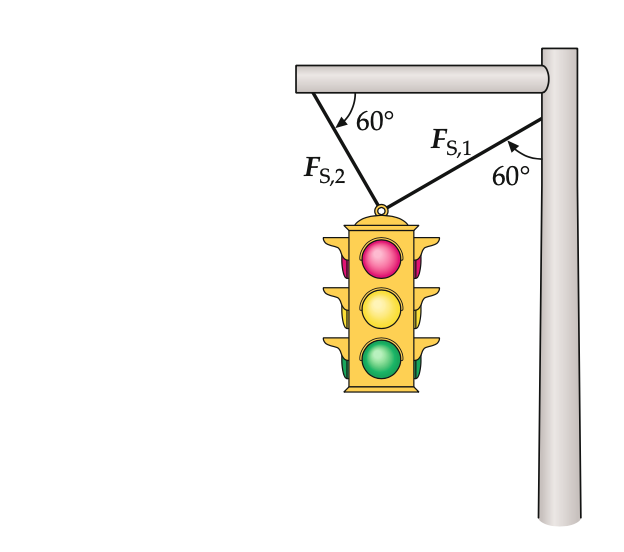
\includegraphics[width=0.5\textwidth]{auf3}
\end{figure}
\pagebreak

\question Ermitteln Sie für die Systeme aus den Abbildung a, b und c, die im Gleichgewicht sind, die unbekannten Zugkräfte und Massen.
\begin{figure}[h]
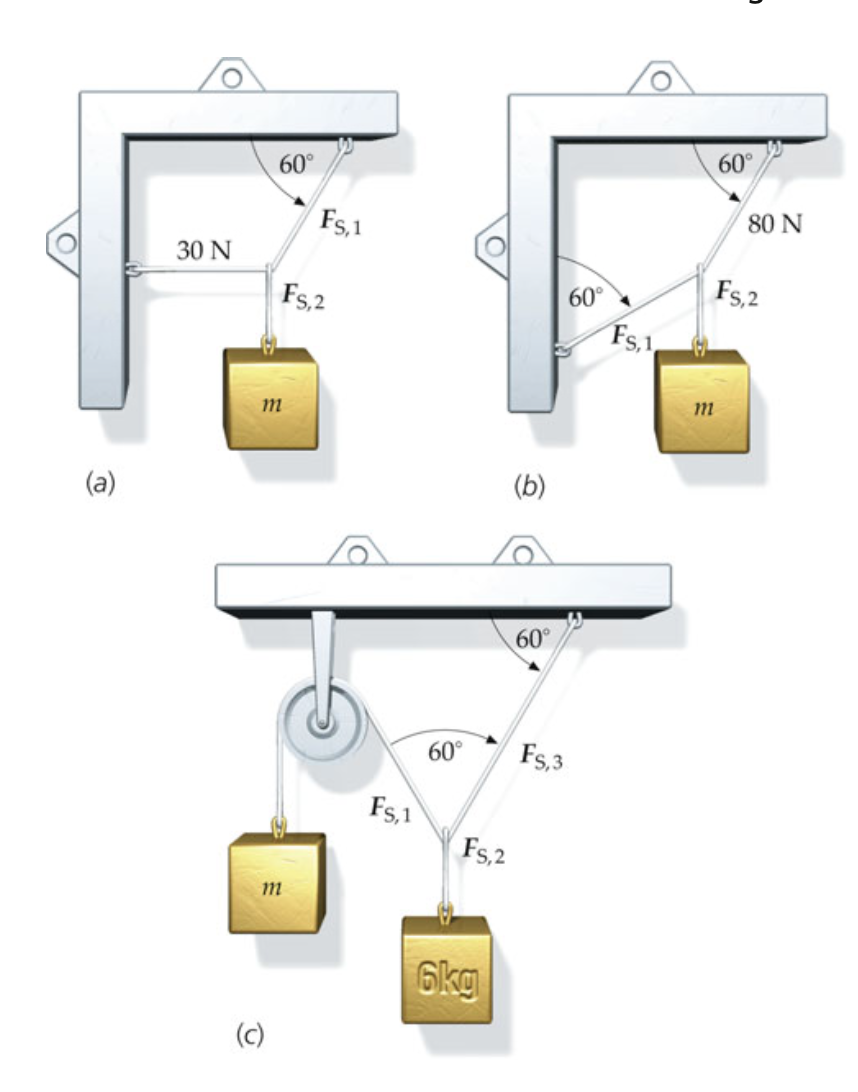
\includegraphics[width=0.6\textwidth]{auf4}
\end{figure}


[Aufgaben  Quelle : Physik für Wissenschaftler und Ingenieure Tipler, Mosca]

\end{questions}

\section*{Mathematik 1}

\begin{questions}
\question Bestimmen Sie in den folgenden Fällen jeweils die Menge aller \(  x \in \mathbb{R} \)  , die den Ungleichungen genügen, und skizzieren Sie diese Mengen auf der Zahlengeraden: 

\begin{figure}[h]
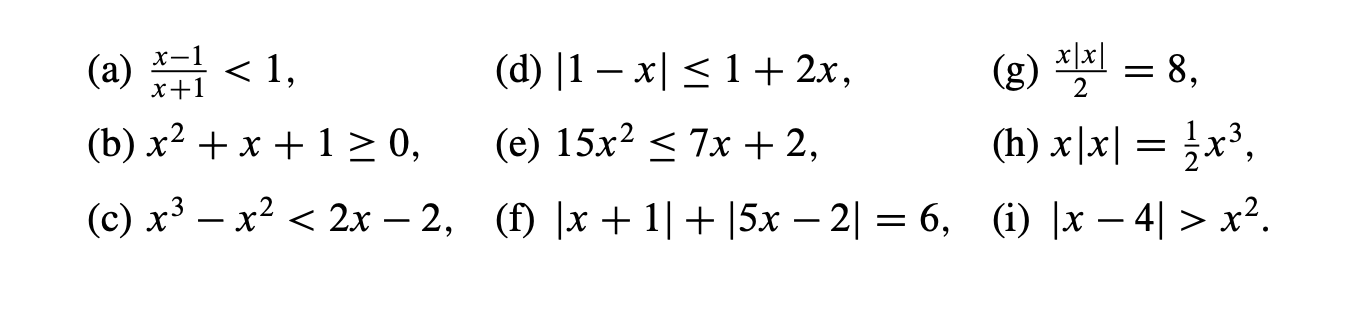
\includegraphics[width=0.7\textwidth]{auf5}
\end{figure}
\end{questions}


\end{document}